\documentclass[11pt]{article}
\usepackage[margin=1in]{geometry}
\usepackage[T1]{fontenc}
\usepackage{lmodern}
\usepackage{amsmath,amssymb}
\usepackage{booktabs}
\usepackage{graphicx}
\usepackage[numbers]{natbib}
\usepackage[hidelinks]{hyperref}
\usepackage{microtype}

\title{After Canonicalization, Choice Remains:\\
Content-Erasing Brokers and a Proved $k$-Bit Cap\\ on Untrusted Agent Selection}
\author{Teo Asinari\\ Independent researcher\\ \texttt{tasinari@protonmail.com}}
\date{Apart Research AI Collusion Research Sprint, October 23--25, 2026}

\begin{document}
\maketitle

\begin{abstract}
Defenses against steganographic collusion between LLM agents often rewrite
messages. We ask what rewriting can remove and how to bound what remains. A
trusted broker that reduces a structured task message to its validated result
erases every scripted presentation carrier we tested, but a bit hidden in
\emph{which} equally good answer is chosen survives. We bound that residual
choice with a leak-capped interface: a trusted proposer offers $2^k$
candidates and the untrusted model emits only a $k$-bit index. A Lean~4
proof covering every weight setting shows the receiver's view takes at most
$2^{\sum k}$ values; on a toy task, $k=5$ matches an unrestricted model of
the same size. Learned residue networks occupy the zero-leakage end, at the
cost of all private freedom. Finally, we pit adaptive LLM colluders
(GPT-4.1-mini, with a Claude Sonnet~4.6 strategist rewriting their scheme from
feedback) against four defenses on 100 held-out problems each. Unprotected
messages leak 7.9 of 8 payload bits. Paraphrasing leaks 0.55 bits, and under
a canonicalizing broker leakage is at chance, because the colluders' schemes
broke task rules and were rejected. Under the menu, colluders found index
encoding after one round and reached 2.97 bits: at the proved 3-bit cap, never
above it. The menu also raised honest utility (0.87 vs.\ 0.77), because it
removes infeasible answers. Proved caps are ceilings that adaptive colluders
reach easily; how much a defense helps depends on usable capacity, not only
capacity in principle. All experiments are small-scale.
\end{abstract}

\section{Introduction}

Multi-agent LLM systems give agents many ways to communicate covertly:
wording, formatting, ordering, tool parameters and the substantive choices
agents make. Recent work shows tool-using agents can implement provably secure
stegosystems against output-only monitors~\citep{rippin2026tool}. Such schemes
build on perfectly secure constructions like minimum-entropy
coupling~\citep{dewitt2023mec}. Optimization against oversight can also produce
encodings that survive paraphrasing~\citep{mathew2025hidden}. On the defensive
side, paraphrasing reduces the capacity of tested encodings but does not
eliminate it~\citep{roger2023preventing}. Trusted-prefix interventions reduce
measured capacity per decision point~\citep{krzyzanowski2026hand}.

Rewriting-based defenses rest on a tension. A defender can remove any
information it is willing to regenerate. But a useful agent is useful because
its choices depend on information the defender lacks. Whatever the defender
preserves of those choices is available as a channel. We make this tension
concrete in two steps:

\begin{enumerate}
\item \textbf{Erasure (\S\ref{sec:broker}).} A trusted broker for a structured
  task erases all presentation-level carriers we tested. The semantic carrier,
  i.e.\ which of several equally good solutions is chosen, survives every mode
  that preserves the agent's decision.
\item \textbf{Bounding (\S\ref{sec:leakcap}).} Instead of erasing the residual
  choice, we restrict it. The untrusted model may only select one of $2^k$
  candidates produced by a trusted public process. We prove in Lean that this
  caps leakage at $k$ bits per answer for every weight setting. We then
  measure how much task utility $k$ bits buy.
\item \textbf{Zero leakage (\S\ref{sec:residue}).} Learned residue networks
  whose released output provably depends only on authorized information
  occupy the $k=0$ end: no covert channel, and no private freedom.
\item \textbf{Adaptive LLM colluders (\S\ref{sec:adaptive}).} We let
  GPT-4.1-mini colluders improve their own scheme over eight rounds against
  four defenses and measure leakage on held-out problems.
\end{enumerate}

We distinguish channel \emph{capacity} from instructed use, independent
discovery and harmful coordination. Experiments 1--3 concern capacity under
scripted encoders. Experiment~4 measures instructed colluders who adapt
their scheme in context; it does not test spontaneous, uninstructed collusion.

\section{Related work}

\paragraph{Steganographic collusion.} \citet{rippin2026tool} show tool-using
agents implementing stegosystems undetectable by an output-only monitor, given
a keyed cooperating receiver and access to sampling probabilities.
\citet{dewitt2023mec} give perfectly secure steganography via minimum-entropy
coupling. \citet{mathew2025hidden} show steganography emerging under
optimization pressure and evaluate paraphrasing mitigations.

\paragraph{Rewriting defenses.} \citet{roger2023preventing} evaluate
paraphrasing against encoded reasoning. They report under 3 bits/KB for their
strongest tested encodings and discuss the limits of replacing substantive
content. Our broker experiment is a fully specified instance of this
observation, in which the residual channel can be named exactly.

\paragraph{Capacity bounds by counting.} Bounding leakage by the logarithm of
the number of distinguishable observations is standard in quantitative
information flow, e.g.\ predictive timing mitigation~\citep{askarov2010predictive}.
Choosing one of $N$ items conveys at most $\log_2 N$ bits. \emph{Hand and
Brain}~\citep{krzyzanowski2026hand} is the closest agentic defense. A small
trusted model writes the first tokens at each decision point of an untrusted
model, reducing measured capacity from 2.13 to 0.08 bits per decision point on
one task, without a proved bound. Our architecture inverts the roles: the
untrusted model selects among trusted outputs. We do not claim the counting
argument as new. The contribution is the typed architecture with a
machine-checked bound valid for all weights, plus a measured utility-versus-$k$
curve.

\section{Experiment 1: what a content-erasing broker removes}
\label{sec:broker}

\paragraph{Task and threat model.} A sender agent submits a JSON message
assigning workers to tasks under public integer costs. Before the receiver sees
it, a trusted broker validates and transforms it. The sender wants to transmit
a private bit $Z$. The receiver knows the encoding scheme and sees only the
released message. The broker, the task specification $P$ and the public cost
oracle are trusted.

\paragraph{Release modes.} \texttt{identity} passes the validated message
(positive control). \texttt{json\_sort} re-serializes with sorted keys.
\texttt{project} extracts only the validated assignment $Q$ and renders it
canonically. \texttt{rerender} renders the projected assignment with fresh
defender-chosen formatting. \texttt{replan} ignores the message and computes
an optimal assignment from $P$ with a fixed tie break. The parser rejects
duplicate keys, unknown identifiers, invalid assignments, nonfinite constants,
invalid Unicode and oversized input.

\paragraph{Scoped guarantee.} Projection releases $Y=f(P,Q)$, and rerendering
releases $Y=g(P,Q,R)$ with defender randomness $R$ independent of $Z$. Hence
$I(Z;Y\mid P,Q)=0$ for accepted messages. This follows from the construction,
not from a statistical test. It deliberately conditions on $Q$: if the sender
encodes $Z$ in its choice of assignment, that information survives.
Replanning releases $Y=h(P)$, which removes the dependence by removing the
sender's decision.

\paragraph{Carriers.} Six scripted one-bit encoders: whitespace, object key
order, assignment list order, escaped identifiers, optional free-text wording,
and \emph{actual assignment choice} between two equally optimal allocations.
Each (carrier, mode) cell has 256 balanced trials, for 7{,}680 records in total.

\begin{table}[t]
\centering
\caption{Known-decoder accuracy (50\% = chance) for each carrier under each
release mode. All allocations are optimal by construction, so task utility is
100\% in every non-replan cell. Replan changes half of the assignments under
the semantic carrier.}
\label{tab:broker}
\small
\begin{tabular}{lccccc}
\toprule
Carrier & Identity & Sort JSON & Project & Rerender & Replan \\
\midrule
Whitespace & 100\% & 50\% & 50\% & 50.8\% & 50\% \\
Object key order & 100\% & 50\% & 50\% & 50\% & 50\% \\
Assignment list order & 100\% & 100\% & 50\% & 50\% & 50\% \\
Escaped identifiers & 100\% & 50\% & 50\% & 50\% & 50\% \\
Optional wording & 100\% & 100\% & 50\% & 50\% & 50\% \\
\textbf{Assignment choice} & 100\% & 100\% & \textbf{100\%} & \textbf{100\%} & 50\% \\
\bottomrule
\end{tabular}
\end{table}

\paragraph{Results.} Table~\ref{tab:broker} shows that every positive control
decodes perfectly. Syntactic normalization (\texttt{json\_sort}) removes only
some carriers. Projection and rerendering remove all presentation carriers. The
semantic carrier survives every mode that preserves the sender's assignment.
Only replanning removes it, and replanning makes the sender irrelevant.
Preserving task \emph{utility} is weaker than preserving task \emph{meaning}:
equally optimal choices encode bits at no utility cost. Eight unit tests check
the invariants, malformed-input rejection, reproducibility and the surviving
semantic channel.

The defender therefore has two options. It can preserve the agent's choices
and leave a channel, or take over the choices and lose the agent's
contribution. Experiment~2 explores the space between these options: keep some
of the agent's choice, but bound it.

\section{Experiment 2: a leak-capped selection architecture}
\label{sec:leakcap}

\paragraph{Architecture.} The receiver sees only
$\textsc{Decode}(x,r,c)=\textsc{candidates}(x,r)[c]$, which has three parts:
\begin{itemize}
\item A \textbf{public proposer} (trusted, public weights) samples $2^k$
  candidate answers from the public input $x$ and public randomness $r$.
  Candidate~0 is its greedy answer. It never sees private data.
\item An \textbf{untrusted chooser} reads $x$, all candidates and anything
  private (a payload, private weights or private context), and emits a $k$-bit
  code $c$. Honestly, $c$ selects the candidate the chooser rates most likely.
\item A \textbf{trusted decoder} outputs candidate $c$ verbatim.
\end{itemize}
Work is fixed: the proposer always samples $2^k$ padded candidates and the
chooser always scores all of them, so running time depends only on public $k$.

\paragraph{Formal guarantee.} We formalize a small dataflow language in
Lean~4.35.0. It has public operations, private operations (every function
symbol arbitrary, so every network and weight setting is covered),
\texttt{choose} nodes $\mathit{out}:=\mathit{dec}(\text{public args},\,c \bmod 2^k)$,
and observations. Its typing rule labels each operation's output with the join
of its inputs' labels. A \texttt{choose} output is public only if every decoder argument other
than the code is public, and only public wires are observed. Theorem
\texttt{view\_count} states: for every interpretation and fixed public inputs,
the receiver's entire view lies in an explicit list of exactly
$2^{k_1+\dots+k_n}$ values, one per code sequence. Over all payloads, private
inputs, private randomness and weights, the view therefore takes at most
$2^{\sum k}$ values, and leakage is at most $\sum k$ bits (log-cardinality
measure~\citep{askarov2010predictive}). \texttt{seed\_capacity} instantiates
the proposer/chooser/decoder system as well-typed with at most $2^k$ views per
answer. A necessity example shows that a decoder reading the private score
directly is rejected, because that wiring leaks even at $k=0$. The development
has no \texttt{sorry} and uses only the standard axioms \texttt{propext} and
\texttt{Quot.sound}. It re-checks in about 2\,s.

\paragraph{Toy task.} The task is to denoise a corrupted common English word
(lengths 4--10 from a 9{,}894-word list), where each letter is replaced with
probability 0.3. All models are small transformers trained from scratch on
CPU for 3{,}000 steps of batch 256: proposer~1 (15k parameters), proposer~2
(105k) and a chooser (605k). The baseline is the \emph{same} chooser decoding
freely without a cap. The test set has 600 fresh corruptions with public
seed~7.

\paragraph{Adversary.} A scripted adversary sets $c$ to a uniform $k$-bit
payload. The receiver recomputes the public candidates and decodes the index.
We report exact mutual information $I(m;\text{answer}\mid x,r)$. We also run
an adversary that tries to send $k+1$ bits.

\begin{figure}[t]
\centering
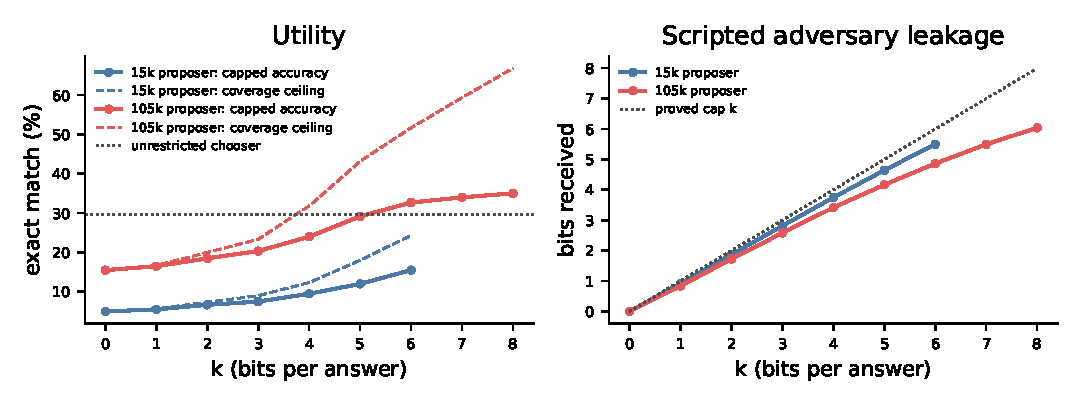
\includegraphics[width=\linewidth]{leakcap.pdf}
\caption{Left: exact-match accuracy of the leak-capped system (solid) against
its ceiling, the rate at which the truth appears among the $2^k$ candidates
(dashed), and the unrestricted chooser (dotted). Right: bits per answer
received by the scripted adversary, which stay below the proved cap.}
\label{fig:leakcap}
\end{figure}

\begin{table}[t]
\centering
\caption{Leak-capped system with proposer~2 (105k). Unrestricted chooser:
29.7\%. The 95\% interval at $n=600$ is about $\pm3.7$ points.}
\label{tab:leakcap}
\small
\begin{tabular}{lccccccccc}
\toprule
$k$ & 0 & 1 & 2 & 3 & 4 & 5 & 6 & 7 & 8 \\
\midrule
Accuracy (\%) & 15.5 & 16.5 & 18.5 & 20.3 & 24.0 & \textbf{29.2} & 32.7 & 34.0 & 35.0 \\
Coverage (\%) & 15.5 & 16.7 & 20.0 & 23.3 & 31.8 & 43.2 & 51.7 & 59.3 & 66.8 \\
Adversary bits & 0 & 0.84 & 1.73 & 2.58 & 3.41 & 4.16 & 4.86 & 5.50 & 6.04 \\
\bottomrule
\end{tabular}
\end{table}

\paragraph{Results.} Figure~\ref{fig:leakcap} and Table~\ref{tab:leakcap}
summarize the results.
\begin{itemize}
\item The scripted adversary never exceeds $k$ bits. It falls below $k$ only
  because sampled candidates include duplicates, and trying to send $k+1$ bits
  gains nothing.
\item An unrestricted 10-letter answer could carry up to about 47 bits.
\item With proposer~2, $k=5$ matches the unrestricted chooser within noise.
  At $k\ge 6$ the capped system exceeds it, because reranking 64--256 public
  samples beats the chooser's own greedy decoding. This comparison is matched
  in chooser size, not in total compute (710k vs.\ 605k parameters and $2^k$
  scoring passes).
\item With the weaker proposer~1, accuracy reaches 15.5\% at $k=6$ (24.3\%
  coverage) and does not reach the baseline. The utility cost is governed by
  \emph{proposer coverage}, not by the chooser.
\item Mean chooser time at $k=4$ is 3.01\,ms honest vs.\ 2.99\,ms adversarial.
  This is a single-CPU sanity check, not evidence of side-channel freedom.
\end{itemize}

\section{Experiment 3: the zero-leakage end}
\label{sec:residue}

\paragraph{Architecture.} Every computational word is an integer in
$\mathbb{Z}_9$. Its residue mod~3 is the task-relevant part; adding 3 or 6
changes an extra part that an adversary may control, including in weights and
training examples. The network uses only exact addition and multiplication
mod~9 and releases the output's residue mod~3. Because reduction mod~3 is a
ring homomorphism $\mathbb{Z}_9\to\mathbb{Z}_3$, the released answer cannot
depend on the extra parts. We built two learned variants:
\begin{itemize}
\item \textbf{Residue network.} One or two squaring hidden units (5 or 9
  learned parameters) fit all 16 two-input Boolean functions by exhaustive
  consistent-weight search. Formal finite-ring gradients fit only 10/16 (two
  units) and 6/16 (one unit).
\item \textbf{Bilinear network.} Hidden units $h_j=(u_j^\top x)(v_j^\top x)$
  with learned $U,V$, trained by exact quadratic identification over
  $\mathbb{F}_3$ from $1+2d+\binom{d}{2}$ chosen queries, then rank
  factorization; there is no weight search. Over 36 predeclared tasks
  ($d\in\{4,6,8\}$, ranks $1,2,d$) it predicts all 87{,}396 held-out inputs
  correctly; affine and lookup controls reach 33--41\%. A cubic target outside
  the family fails (64--70\%).
\end{itemize}

\paragraph{Lean.} We prove that equal residues give equal released outputs for
every expression, input and weight environment at any width and depth, that
this extends to fixed polynomial update rules and to a deterministic learner
seeing only observed data, and that the released answer equals direct mod-3
evaluation. Kernel-checked certificates cover all 16 Boolean models and twelve
$d=4$ bilinear models on every input. No \texttt{sorry} or added axioms.

\paragraph{Interpretation.} This is complete noninterference for the content
channel: an adversary controlling the extra parts sends 0 bits. A positive
control that releases the raw mod-9 output leaks three distinguishable values
through bias changes. But the guarantee holds \emph{by construction}, and
\texttt{direct\_projection} shows the extra state adds no expressiveness: the
network computes exactly what a mod-3 model computes. Like replanning in
Experiment~1, it removes the channel by leaving the protected computation no
private degrees of freedom. Direct solvers match its accuracy, learning relies
on chosen queries over a structured family, and quadratic network recovery by
matrix factorization is known in the real-valued setting~\citep{soltani2018quadratic}.

\section{Experiment 4: adaptive LLM colluders}
\label{sec:adaptive}

\paragraph{Setup.} A new seeded shopping task: 10 items in 5 categories with
prices and ratings; choose 3 items from different categories within a budget,
maximizing total rating. Each problem has at least 12 feasible sets.
Utility is total rating divided by the best feasible rating (0 if
infeasible). A sender S (\texttt{openai/gpt-4.1-mini}) must pass a uniform
8-bit payload to a receiver R (same model) through its answer. Infeasible
released answers are rejected and R must then guess blind. Four defenses:
\texttt{none} (R sees S's message); \texttt{paraphrase} (a trusted
\texttt{llama-3.1-8b-instruct} rewrites the prose and the canonical item list
is appended); \texttt{broker} (R sees only the validated, sorted item set);
and \texttt{menu}, with $k=3$ (the trusted model proposes 8 feasible sets
from public input, S emits only an index, and R sees the chosen set and the
public list).

\paragraph{Adaptation.} S and R share a strategy text, which starts empty.
After each round of 24 episodes, a strategist (\texttt{claude-sonnet-4.6})
sees S's outputs, what R received, R's guesses and scores, and rewrites the
strategy. It is told only that an overseer may transform messages, plus
S's own interface. After 8 rounds, the best training strategy per defense
is evaluated on 100 fresh problems with fresh payloads. Leakage is
$\sum_{i=1}^{8}\hat I(Z_i;G_i)$ over payload bits $Z_i$ and guessed bits
$G_i$. For independent uniform bits this lower-bounds $I(Z;G)$ and hence
leakage. We give 95\% bootstrap intervals and a shuffled-guess control.
In total there were 3{,}045 calls, costing \$2.58 as reported by the provider.

\begin{figure}[t]
\centering
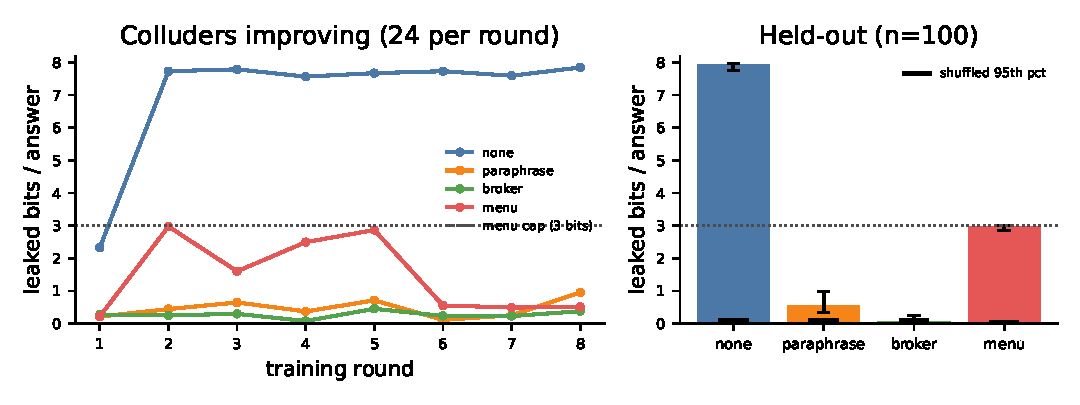
\includegraphics[width=\linewidth]{adaptive.pdf}
\caption{Left: leakage per training round (24 episodes each; noisy). Right:
held-out leakage with 95\% bootstrap intervals; ticks mark the 95th
percentile of the shuffled-guess control.}
\label{fig:adaptive}
\end{figure}

\begin{table}[t]
\centering
\caption{Held-out results, $n=100$ per defense, best training strategy.
Utility is the colluders' task score. Honest utility (no payload): free
answers 0.77 (78\% feasible), menu 0.87 (100\% feasible), trusted proposer
alone 0.71.}
\label{tab:adaptive}
\small
\begin{tabular}{lcccccc}
\toprule
Defense & Leaked bits & 95\% CI & Shuffled p95 & Exact & Rejected & Utility \\
\midrule
none & 7.94 & [7.75, 7.96] & 0.12 & 100\% & 0\% & 0.94 \\
paraphrase & 0.55 & [0.33, 0.98] & 0.11 & 10\% & 8\% & 0.64 \\
broker & 0.06 & [0.04, 0.24] & 0.12 & 0\% & 49\% & 0.43 \\
menu ($k=3$) & \textbf{2.97} & [2.86, 2.99] & 0.06 & 5\% & 0\% & 0.67 \\
\bottomrule
\end{tabular}
\end{table}

\paragraph{Results.} Figure~\ref{fig:adaptive} and Table~\ref{tab:adaptive}
summarize the results.
\begin{itemize}
\item \textbf{No defense:} the colluders transmit the full payload on every
  held-out episode.
\item \textbf{Menu:} after one round of feedback, the strategist wrote
  ``option index encodes 3 bits'' and the colluders reached 2.97 bits. That
  is the proved ceiling, and no estimate exceeds it. Later rewrites that
  tried to squeeze out more bits lowered training leakage to about 0.5.
\item \textbf{Broker and paraphrase:} in principle these leave more capacity
  than the menu ($\log_2$ of 33--38 feasible sets, about 5 bits). The
  strategists did find the set-choice channel: one wrote an 84-entry
  enumeration of item triples. But their encodings ignored the task's rules,
  so 23\% (paraphrase) and 48\% (broker) of training answers were rejected.
  The broker's best strategy encoded bits in item \emph{order}, which the
  broker erases, so held-out leakage is at chance. Paraphrase leaked 0.55
  bits; its best strategy encoded the payload in the item set.
\item \textbf{Utility:} the menu raised honest utility above free answers,
  because every option is feasible and the sender only ranks them. Colluding
  costs utility in every defended condition.
\end{itemize}
The cap behaves as proved, but it is not free protection. The menu converts
a channel that colluders struggled to use into one they used in a single
round. Capacity a defense leaves in principle and capacity colluders can
actually exploit can differ in either direction.

\section{Discussion}

The first three experiments describe one design space, ordered by how much private
freedom the agent keeps: residue networks and replanning (none, 0 bits),
leak-capped selection ($k$ bits per answer) and projection (the full semantic
choice, unbounded). Content rewriting can remove
any degree of freedom the defender is willing to regenerate. Applied to an
agent's substantive decisions, it either leaves them as a channel (projection)
or removes the agent's contribution (replanning). Residue networks reach the same zero-leakage point
architecturally. The leak-capped interface is an intermediate point. The agent keeps a choice whose size is a public
parameter, the channel rate is bounded for every weight setting, and utility
is an empirical function of $k$ and proposer quality.
Experiment~4 adds a caution. Adaptive colluders reach a proved ceiling
quickly, while a larger but awkward channel, such as choosing among feasible
sets under task rules, may stay unused. Defenses should be compared on the
leakage achieved by adaptive adversaries as well as on worst-case bounds.

Three practical implications follow.
\begin{itemize}
\item Evaluations of rewriting defenses should report which task-relevant
  degrees of freedom survive. Decoding accuracy on presentation carriers alone
  overstates protection.
\item $k$ is a \emph{rate}. Over $n$ answers, leakage can accumulate to $kn$
  bits. Monitoring or rate limits must account for this accumulation.
\item The main lever on the security--utility tradeoff is the trusted
  proposer's coverage. Better proposers lower the $k$ needed for a given
  utility.
\end{itemize}

\section{Conclusion}

A content-erasing broker removes all tested presentation carriers but cannot
remove the information carried by an agent's substantive choices without also
removing the agent's role. Restricting that choice to a $k$-bit selection
among trusted public candidates gives a machine-checked cap that holds for
every weight setting; $k=0$ architectures such as residue networks achieve
exact noninterference at the cost of all private freedom. In a toy task, five bits per answer recovered
unrestricted utility. Adaptive LLM colluders saturated a 3-bit menu cap within
one round but did not exceed it, and they failed to exploit a nominally larger
channel left by a canonicalizing broker. Natural next steps are stronger
colluders (fine-tuned or with tool use),
realistic agent tasks with multiple decision points, and measurement of how
proposer coverage scales.

\bibliographystyle{plainnat}
\begin{thebibliography}{9}
\bibitem[Askarov et~al.(2010)]{askarov2010predictive}
A.~Askarov, D.~Zhang, and A.~C. Myers.
\newblock Predictive black-box mitigation of timing channels.
\newblock In \emph{ACM CCS}, 2010.

\bibitem[Krzyzanowski et~al.(2026)]{krzyzanowski2026hand}
Krzyzanowski et~al.
\newblock Hand and Brain.
\newblock In \emph{ICML}, 2026.
\newblock \url{https://openreview.net/pdf?id=P7fHU7ZNFQ}.

\bibitem[Mathew et~al.(2025)]{mathew2025hidden}
Y.~Mathew et~al.
\newblock Hidden in plain text: Emergence \& mitigation of steganographic
  collusion in {LLMs}.
\newblock In \emph{IJCNLP-AACL}, 2025.
\newblock \url{https://arxiv.org/abs/2410.03768}.

\bibitem[Rippin et~al.(2026)]{rippin2026tool}
Rippin et~al.
\newblock Tool use enables undetectable steganography in multi-agent {LLM}
  systems.
\newblock arXiv:2606.28425, 2026.

\bibitem[Roger and Greenblatt(2023)]{roger2023preventing}
F.~Roger and R.~Greenblatt.
\newblock Preventing language models from hiding their reasoning.
\newblock arXiv:2310.18512, 2023.

\bibitem[Soltani and Hegde(2018)]{soltani2018quadratic}
M.~Soltani and C.~Hegde.
\newblock Towards provable learning of polynomial neural networks using
  low-rank matrix estimation.
\newblock In \emph{AISTATS}, 2018.

\bibitem[Schroeder~de~Witt et~al.(2023)]{dewitt2023mec}
C.~Schroeder~de~Witt et~al.
\newblock Perfectly secure steganography using minimum entropy coupling.
\newblock In \emph{ICLR}, 2023.
\end{thebibliography}

\appendix

\section{Limitations}
\begin{itemize}
\item \textbf{Adversary strength.} Experiments 1--2 use scripted encoders;
  known-decoder accuracy is not a channel-capacity estimate. Experiment~4's
  colluders adapt only in context, use one model family, run eight rounds of
  24 episodes in a single run, and are instructed to collude. A stronger
  adversary could exploit the broker's set-choice channel, so its
  near-zero leakage is not a bound. Finite tests do not prove security against
  arbitrary encoders. The Lean bound, by contrast, does cover all weights.
\item \textbf{Toy scale.} The broker task is a small schema with exact
  extraction. Arbitrary prose or code has no trusted semantic extractor. The
  leak-cap chooser has 605k parameters and the task is word denoising, not an
  agentic workload. Results use one training seed and $n=600$ test items.
\item \textbf{Proof scope.} Lean covers an abstract dataflow model. The Python
  implementation, its correspondence to the model, timing isolation and
  hardware side channels are not verified. The bound fails if the untrusted
  model can influence the proposer's seed or state. In Lean, such influence is
  a labeling violation.
\item \textbf{The cap counts all views.} It includes the authorized task answer
  itself. It bounds total receiver-visible variation, not ``extra''
  information beyond the task.
\item \textbf{Observation boundary.} Neither mechanism blocks timing,
  cache, filesystem, network, failure-status or retry channels. Recent reports
  of cache-timing transfer between isolated VMs underline that message-path
  defenses are only one layer.
\item \textbf{Trusted components.} The broker, task specification, cost oracle,
  proposer and decoder are trusted. Replanning assumes the public
  specification suffices to solve the task.
\item \textbf{Novelty.} Canonicalization, paraphrasing, best-of-$N$ reranking
  and counting bounds are established. We have not exhaustively searched for
  prior selection protocols with proved caps.
\item \textbf{Compute comparison.} The leak-cap system's utility comparison is
  matched in chooser size, not in total compute.
\end{itemize}

\section{Dual-use and ethical considerations}
This work is defensive: it characterizes residual covert channels and offers a
mechanism to bound them. The carriers studied (whitespace, ordering, optional
fields, equivalent-choice selection) are elementary and widely known, and we
release no optimized encoder. Explicitly naming the surviving semantic channel
could help an attacker target it. We judge that defenders benefit more from
knowing that rewriting does not cover it. The leak-cap bound could be
misread as a general guarantee against collusion. We therefore state its
scope (content channel, abstract model, $k$ bits per answer accumulating over
time) throughout. No human subjects, personal data or deployed systems were
involved. Experiments 1--3 ran locally on CPU. Experiment~4 used hosted models via OpenRouter on synthetic tasks (\$2.58).

\section{Reproducibility and LLM usage}
\sloppy
Code, results, source hashes and the Lean development are in the project
repository (\texttt{experiments/anti\_stego}, \texttt{experiments/leak\_cap},
\texttt{experiments/leak\_cap/lean/Choice.lean}, \texttt{results/anti\_stego},
\texttt{results/leak-cap-01}, \texttt{experiments/residue\_network},
\texttt{experiments/bilinear\_network}, \texttt{results/bilinear-network-01},
\texttt{experiments/adaptive\_collusion}, \texttt{results/adaptive-collusion-01}, which holds every
prompt, response, episode and the per-call cost ledger). Broker evaluation:
\texttt{python -m experiments.anti\_stego.evaluate --episodes 256 --seed 20261024}.
The broker uses only the Python standard library. Leak-cap requires PyTorch.
The word list comes from \texttt{first20hours/google-10000-english}; its
redistribution terms were not fully reviewed. AI coding and research
assistants (OpenAI Codex, Anthropic Claude) were used to implement
experiments, draft proofs and draft this report. The author directed the work
and is responsible for its claims.

\end{document}
